%%=============================================================================
%% Inleiding
%%=============================================================================

\chapter{Inleiding}
\label{ch:inleiding}

%De inleiding moet de lezer alle nodige informatie verschaffen om het onderwerp te begrijpen zonder nog externe werken te moeten raadplegen \autocite{Pollefliet2011}. Dit is een doorlopende tekst die gebaseerd is op al wat je over het onderwerp gelezen hebt (literatuuronderzoek).

%Je verwijst bij elke bewering die je doet, vakterm die je introduceert, enz. naar je bronnen. In \LaTeX{} kan dat met het commando \texttt{$\backslash${textcite\{\}}} of \texttt{$\backslash${autocite\{\}}}. Als argument van het commando geef je de ``sleutel'' van een ``record'' in een bibliografische databank in het Bib\TeX{}-formaat (een tekstbestand). Als je expliciet naar de auteur verwijst in de zin, gebruik je \texttt{$\backslash${}textcite\{\}}.
%Soms wil je de auteur niet expliciet vernoemen, dan gebruik je \texttt{$\backslash${}autocite\{\}}. Hieronder een voorbeeld van elk.

%\textcite{Knuth1998} schreef een van de standaardwerken over sorteer- en zoekalgoritmen. Experten zijn het erover eens dat cloud computing een interessante opportuniteit vormen, zowel voor gebruikers als voor dienstverleners op vlak van informatietechnologie~\autocite{Creeger2009}.

%\section{Stand van zaken}
%\label{sec:stand-van-zaken}

%% TODO: deze sectie (die je kan opsplitsen in verschillende secties) bevat je
%% literatuurstudie. Vergeet niet telkens je bronnen te vermelden!

%\lipsum[7-20]

In dit hoofdstuk wordt er een korte inleiding gegeven over de basisprincipes van RAID, aangezien RAID-Z een softwarematige vorm van RAID is. Daarnaast wordt de geschiedenis en globale werking van ZFS reeds kort besproken. Aan het einde van dit hoofdstuk kunnen de probleemstelling en onderzoeksvragen worden teruggevonden, samen met de verdere indeling van deze bachelorproef.

\section{Basisbeginselen van RAID}

Al van oudscher worden magnetische harde schijven gebruikt als opslagmedium voor data \autocite{Goda2012}. Maar reeds in de jaren 80 zagen onderzoekers in dat I/O-performance een bottleneck zou vormen voor computersystemen in de toekomst. Terwijl geheugenchips en processoren steeds sneller werden, bevonden opslagmedia zich in een impasse \autocite{DavidA.Paterson1987}.

In de paper \textit{"A Case for Redundant Arrays of Inexpensive Disks"}  formuleerden \textcite{DavidA.Paterson1987} en zijn collega's voor het eerst de term 'RAID', wat een acroniem is voor 'Redundant Arrays of Inexpensive Disks'. De oorspronkelijke idee achter RAID was dat een verzameling van goedkopere schijven performanter zou zijn dan grotere en duurdere mainframeschijven van die tijd. 

Naast performantie en kost was betrouwbaarheid (reliability)  ook een belangrijke factor. Als bv. één of meerdere schijven van de array falen, dan mag dit geen invloed hebben op de werking van de rest van de verzameling schijven. Daarom introduceerden de onderzoekers de zgn. "RAID levels"    \autocite{DavidA.Paterson1987}, die vandaag de dag nog steeds in gebruik zijn. Er bestaan een aantal RAID-niveaus, waarvan de voornaamste zullen besproken worden.

\begin{figure}
	\centering
	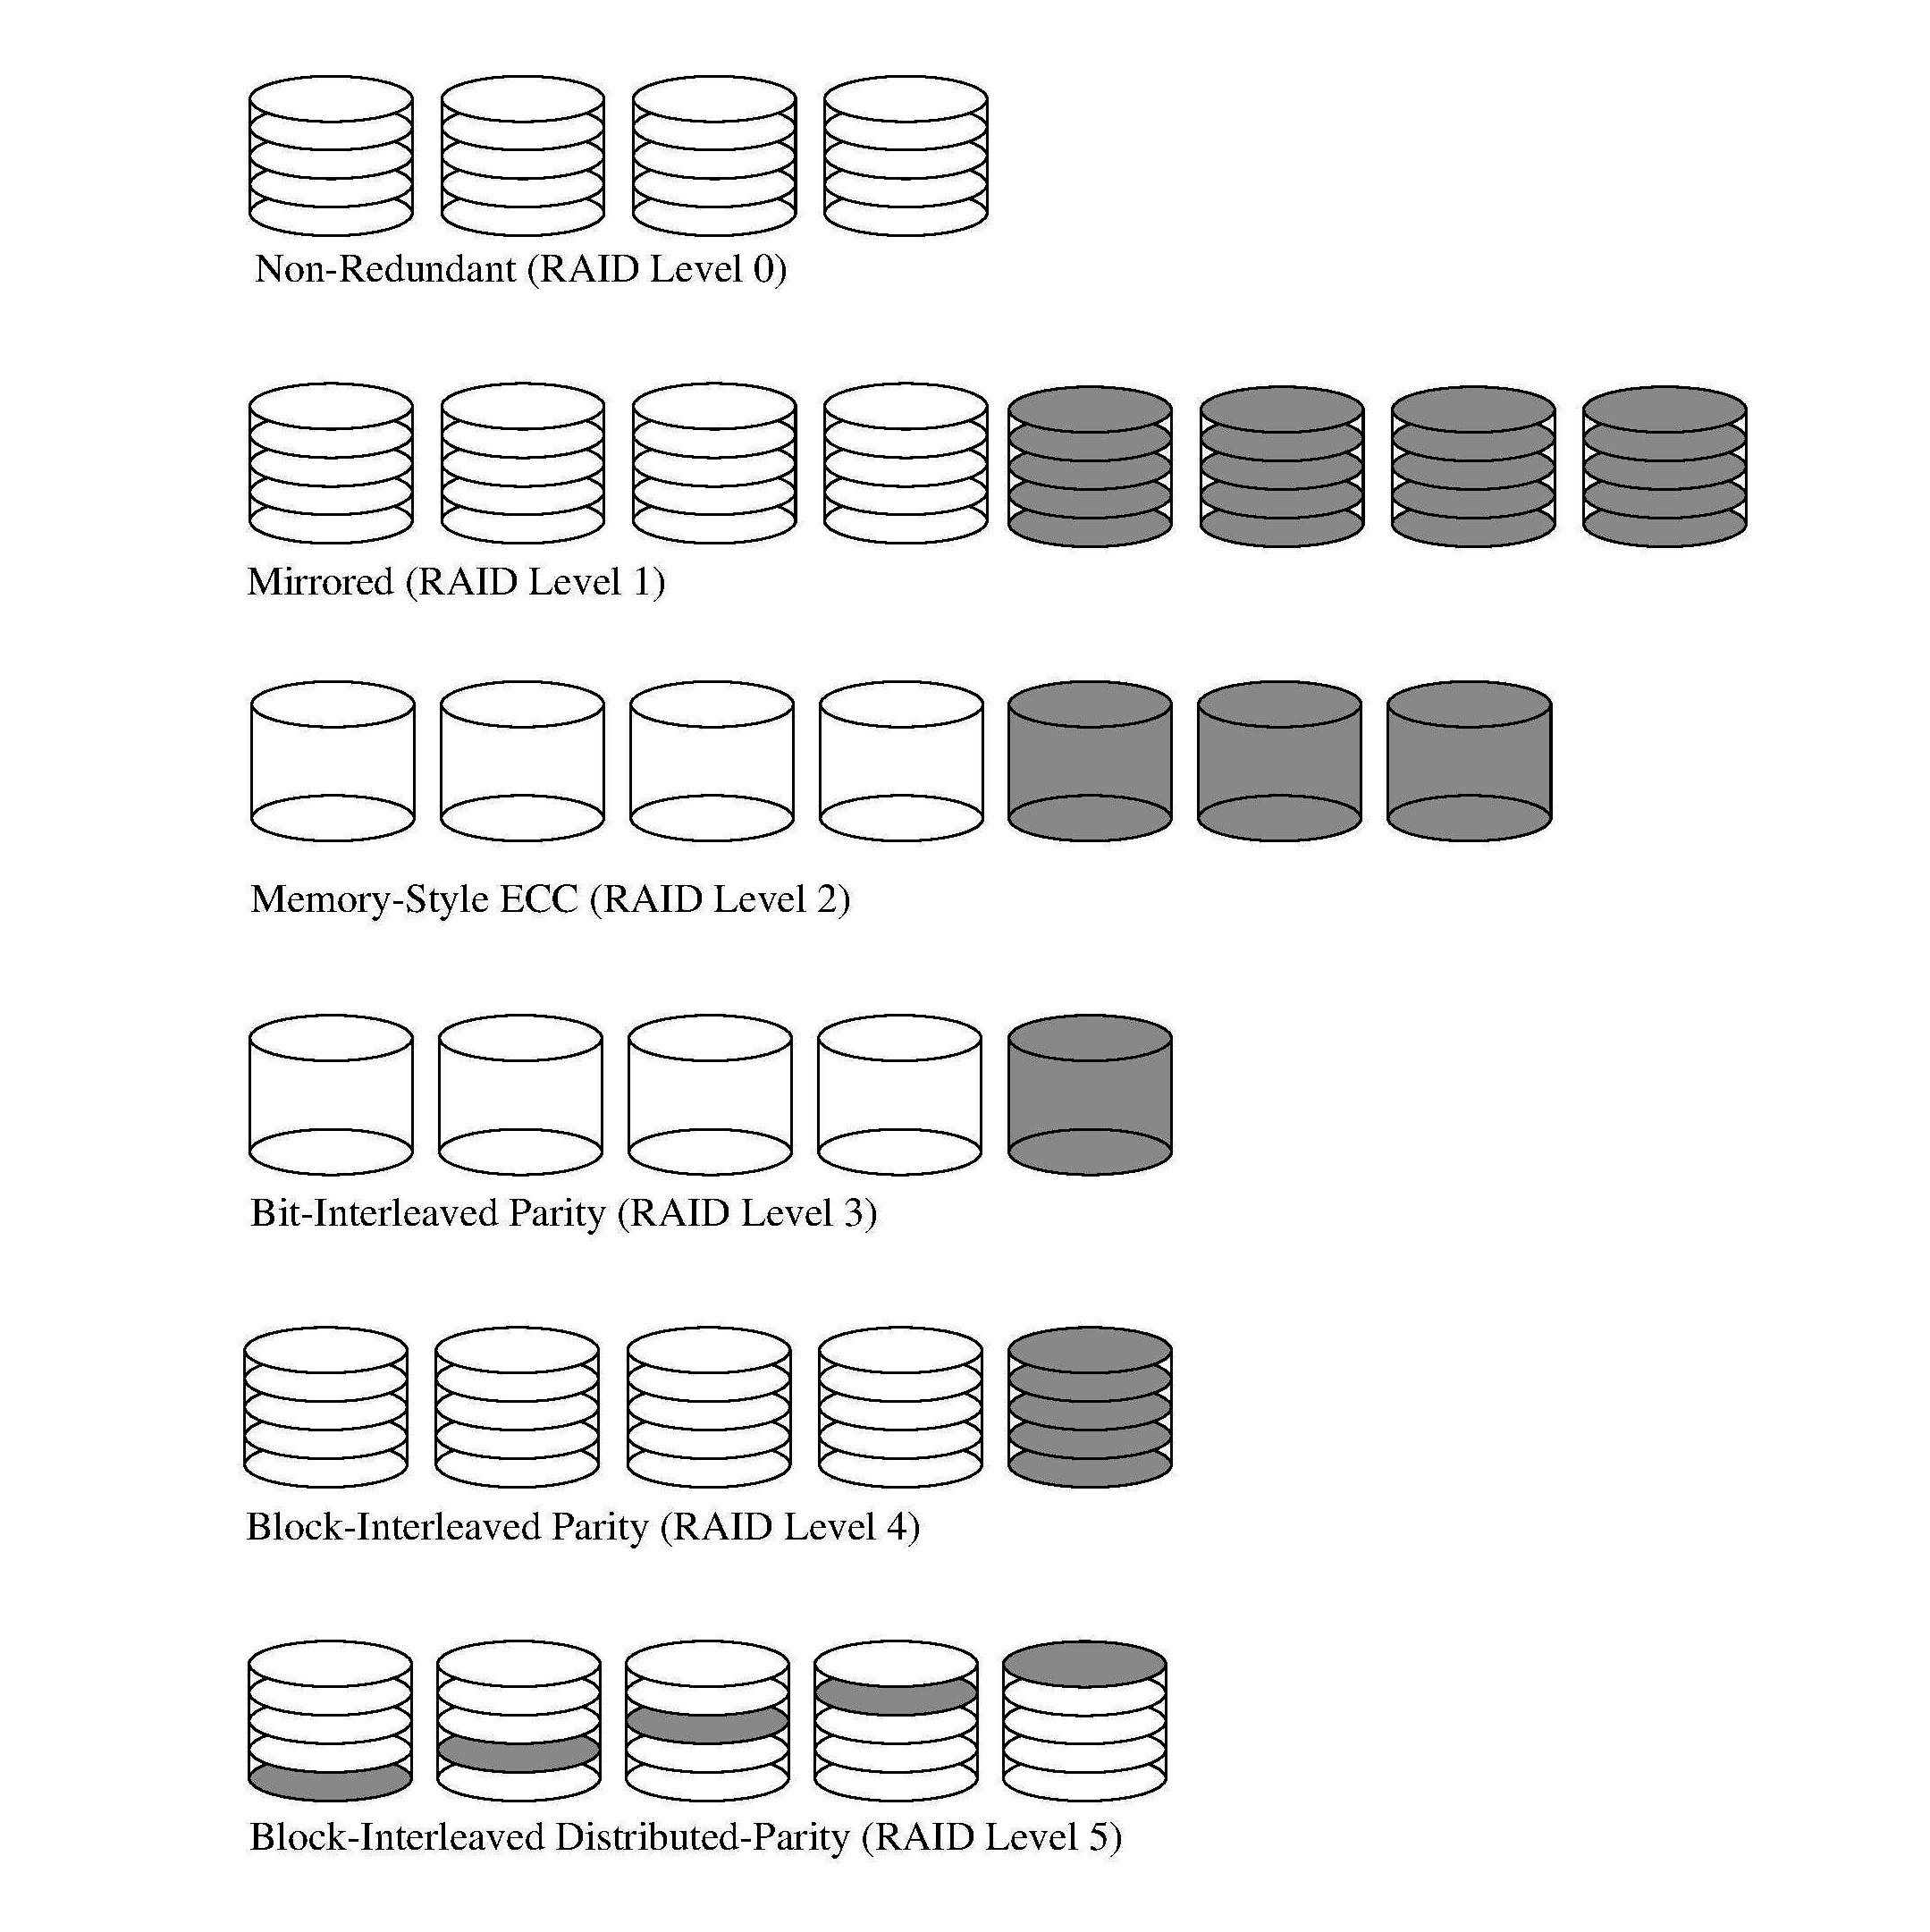
\includegraphics[width=0.8\textwidth]{inleiding-raid-illustratie}
	\caption{Illustratie van verschillende RAID-niveaus \autocite{Chen1994}}
	\label{fig:chen_array_illustratie}
\end{figure}

Bij het bouwen van RAID-systemen worden er gebruikelijk drie aspecten in beschouwing genomen: \textbf{performantie} (performance), \textbf{betrouwbaarheid} (reliability) en \textbf{capaciteit} (capacity). Een RAID-niveau is in principe niets anders dan een balans tussen deze verschillende eigenschappen; meestal zullen er dus één of meerdere trade-offs moeten gemaakt worden \autocite{Chen1994}.

Begrippen die centraal staan bij RAID zijn \textit{\textbf{striping}} en \textit{\textbf{parity}}. Striping heeft betrekking op de manier waarop een RAID-controller (hetzij hardwarematig, hetzij softwarematig) de blokken data verdeelt over de array van schijven. Bij RAID 0 bijvoorbeeld wordt de data gelijkmatig gedistribueerd volgens het \textit{round-robin}-algoritme \autocite{OSThreePiecesRemzi2015}. Datablokken die verdeeld zijn over meerdere schijven en samen één geheel vormen worden een \textit{stripe} genoemd. \\ 
Een voordeel bij RAID 0 is dat de gehele capaciteit van de schijven kan gebruikt worden; er gaat geen ruimte verloren, aangezien de data gelijkmatig verdeeld wordt over de array. Een bijkomend voordeel van striping is dat performantie in het algemeen goed is: de meeste en reads en writes kunnen parallel worden afgehandeld. Een voorwaarde voor goede performantie is echter wel dat de \textit{chunk size} (de grootte van de blokken data die worden weggeschreven en/of uitgelezen) ook optimaal wordt gekozen, i.e. afhankelijk van de workload op het systeem \autocite{OSThreePiecesRemzi2015}. Toch kent RAID 0 een groot nadeel: betrouwbaarheid is nagenoeg onbestaande. Aangezien data nergens wordt gedupliceerd, betekent dat het falen van eender welke disk leidt tot verlies van data \autocite{OSThreePiecesRemzi2015}.

Parity is een mechanisme dat werd geïntroduceerd bij RAID-niveau 4 om betrouwbaarheid af te dwingen. Bij RAID 4 wordt er metadata over de opgeslagen data bijgehouden in parity blocks op een aparte schijf. Deze metadata wordt verkregen d.m.v. het uitvoeren van een mathematische functie op de opgeslagen data. Meestal is dit een XOR-functie (exclusieve OF) \autocite{Chen1994}. Aan de hand van deze parity kan bij het verlies van één of meerdere schijven de originele data worden gereconstrueerd door XOR'ing toe te passen op de parity bits en de data bits. Bij een XOR-operatie geven een even aantal enen (1) steeds als resultaat nul (0); omgekeerd geldt ook dat een oneven aantal enen (1) steeds een één (1) als resultaat zullen opleveren. Stel dat één schijf van een array van vier schijven faalt, dan kan nog steeds de originele data worden verkregen. Echter, als er meer dan één schijf verloren gaat, dan is het bij RAID 4 onmogelijk om de originele data te herstellen. Het grote voordeel van RAID 4 is dan weer echter dat er minder wordt ingeboet op capaciteit  dan bij bv. RAID 1 en RAID 5 \autocite{OSThreePiecesRemzi2015}. 

Naast RAID 0 en RAID 4 zijn er nog andere RAID-levels, zoals RAID 1 en RAID 5. RAID 1 staat ook bekend als \textit{mirroring}, omdat het kopieën maakt van de datablokken naar één of meerdere disks afhankelijk van het aantal schijven. Op gebied van capaciteit is RAID 1 niet echt gunstig, aangezien maar de helft van de totale schijfruimte bruikbaar is. Stel dat er vier schijven in een array aanwezig zijn, dan is slechts de opslagcapaciteit van twee schijven bruikbaar. Daarentegen is de betrouwbaarheid van RAID 1 wel vele malen beter dan die van RAID 0: in theorie mogen er bij een reeks van \textit{n} schijven $\frac{n}{2}$ schijven falen. Maar dan mogen de schijven die elkaars mirror zijn niet falen, want dan is de data op deze disks verloren.  Daarom houdt men in de praktijk meestal de maatstaf van één schijf aan \autocite{OSThreePiecesRemzi2015}.

Als laatste wordt RAID 5 besproken. RAID 5 is in principe niets anders dan RAID-niveau 4, maar dan uitgebreid met functionaliteit dat de parity blocks roteert over de verschillende schijven. Dit is een groot verschil t.o.v. RAID 4, waarbij de parity blocks zich op één disk bevinden. Read-performantie is nagenoeg gelijk aan RAID 4, maar write-performantie is stukken beter. Dit komt omdat bij RAID 5 de schrijfoperaties parallel kunnen worden afgehandeld; bij RAID 4 vormt de parity-schijf een \textit{bottleneck} bij het wegschrijven van data \autocite{Chen1994}. De reden hiervoor is dat bij het updaten van data ook de parity blocks moeten worden geüpdatet; alle operaties worden dus m.a.w. serieel uitgevoerd \autocite{OSThreePiecesRemzi2015}.

Er bestaan nog andere, niet-standaard RAID levels, zoals RAID 6 en RAID 10, maar deze worden hier niet besproken.

\section{Inleiding tot ZFS \& RAID-Z}

ZFS is een bestandssysteem dat ontwikkeld is door het toenmalige Sun Microsystems, nu onderdeel van Oracle Corporation. Voormalig Sun-werknemer Jeff Bonwick was de oorspronkelijke hoofdontwikkelaar achter het bestandssysteem. De ontwikkeling van ZFS startte aan het begin van de jaren 2000; Sun had reeds met de ontwikkeling van bestandssystemen geëxperimenteerd, maar deze pogingen misluktten telkens \autocite{Bonwick2015}. ZFS is een \textit{copy-on-write} (COW) bestandssysteem \autocite{BrianHickmann2007}: bij elke aanpassing van een datablok, wordt er eerst een nieuw blok aangemaakt, waarna het aangepaste datablok naar het nieuwe, lege datablok wordt gekopieerd \autocite{ZFSBonwick}.

In die tijd gebruikte het bedrijf haar UNIX-besturingssysteem Solaris intern voor verschillende soorten toepassingen, waaronder file servers \autocite{Bonwick2015}. De schijven van deze servers waren opgedeeld in volumes, beheerd door de Solaris Volume Manager (SVM) en geformatteerd in UFS (UNIX Filesystem) \autocite{Bonwick2015}. Toen een verkeerd ingevoerd SVM-commando erin slaagde om het systeem te doen crashen en voor een enorme \textit{downtime} zorgde bij  Sun, was dit voor Bonwick een aanleiding om volledig \textit{from scratch} een bestandssysteem op te bouwen dat makkelijk in gebruik én beheer was.

De hoofdreden om een volledig nieuw bestandssysteem te ontwikkelen was volgens \textcite{JeffBonwick_lastZFS} dat de toenmalige oplossingen voor bestandssystemen totaal achterhaald waren. Bestandssystemen waren nog ontwikkeld voor opslagnoden uit de jaren '80 en '90, welke niet te vergelijken zijn met de huidige noden van zowel bedrijven als particulieren. Naarmate de nood aan meer opslagruimte steeg, moesten er oplossingen worden bedacht, en dit m.b.v. bestandssystemen die hier helemaal niet op voorzien waren. Een 'tussenoplossing', aldus volgens \textcite{JeffBonwick_lastZFS}, die ook vandaag de dag nog gebruikt wordt, is de combinatie van volumes en bestandssystemen. Volumes zijn abstracties voor (delen van) fysieke schijven; typisch maakt men één bestandssysteem per volume aan. 

%Een andere eigenaardigheid van bestandssystemen is dat deze nog steeds onlosmakelijk zijn verbonden aan een (deel van) een schijf of opslagapparaat. Volume managers zorgen wel voor een zeker niveau van abstractie, maar bestandssystemen blijven nog steeds gekoppeld aan een bepaalde reeks blokken \autocite{ZFSBonwick}. Dit vonden de ontwikkelaars van ZFS nogal omslachtig: zij zijn van mening dat een bestandssysteem een virtuele abstractie van opslagruimte vormt en dus los moet staan van de fysieke blokken op de schijf. \textcite{ZFSBonwick} maakt de vergelijking met het adresseren van RAM geheugen: RAM-geheugen moet ook eerst niet worden geformatteerd en dan apart worden toegewezen aan applicaties. Bij het alloceren en aanspreken van RAM-geheugen is het immers niet nodig voor de applicatie of programmeur om het exacte geheugenadres te kennen; deze taken worden al afgehandeld door memory allocators m.b.v. virtueel geheugen \autocite{ZFSBonwick}.

%Daarom stelden de ZFS-ontwikkelaars \textit{pooled storage} voor, samen met een geïntegreerde volume manager en storage allocator. Een bijkomend voordeel van \textit{pooled storage} is dat bestandssystemen dynamisch kunnen groeien en verkleinen, zonder tussenkomst van de gebruiker, aangezien de opslagruimte van alle disks als één geheel wordt gezien i.p.v. afzonderlijke eenheden. ZFS maakt het wel mogelijk om quota's in te stellen op bestandssystemen, opdat één bestandssystemen niet alle beschikbare ruimte zou innemen \autocite{ZFSBonwick}. 

Het ZFS-bestandssysteem omvat ook een softwarematige RAID, RAID-Z genaamd. Volgens \textcite{Bonwick2005} lost RAID-Z in combinatie met ZFS een aantal problemen op die inherent aanwezig zijn bij andere RAID-implementaties. Zo claimen de ontwikkelaars dat RAID-Z het zogenaamde RAID5 \textit{write hole} probleem volledig oplost. Bij klassieke RAID-oplossingen worden stripes weggeschreven op een niet-atomaire manier, i.e. de bewerkingen worden niet als één geheel uitgevoerd. Een bijkomend probleem hierbij is dat bij RAID-levels met \textit{parity} (zoals RAID5) ook nog eens de parity-blocks moeten herberekend worden. Indien het systeem tussen deze bewerkingen crasht of uitvalt door bv. elektriciteitsproblemen, dan bevindt de data op de array van schijven zich in een inconsistente toestand: stripes en parity blocks kunnen corrupt raken \autocite{Bonwick2005}. 

%Een oplossing voor dit probleem is het gebruik van NVRAM waarin stripes tijdelijk kunnen worden bijgehouden. Indien er zich dan een systeemcrash voordoet, dan kan de RAID-controller m.b.v. de gegevens in het NVRAM de originele data herstellen. Maar waar RAID geen oplossing voor heeft, aldus volgens \textcite{Bonwick2005}, is het optreden van \textit{silent data corruption}; de RAID-controller weet immers niet of het al dan niet om corrupte data gaat. Het enige waar een RAID-controller zicht op heeft, zijn blokken. Hiervoor biedt ZFS samen met RAID-Z een oplossing: aangezien het bestandssysteem en RAID-Z samen één geheel vormen, is het mogelijk om van datacorruptie te herstellen of om dit zelfs tegen te gaan. Bij het herstellen van data op de array, overloopt RAID-Z de metadata van het bestandssysteem om zo de stripe-grootte te achterhalen. Ook vergelijkt ZFS bij elk datablok de berekende checksum: indien deze checksums niet overeenkomen, dan tracht ZFS dit blok te repareren m.b.v. de parity-informatie van RAID-Z. Op deze manier kan datacorruptie vroegtijdig worden opgemerkt en kan defecte hardware eventueel vervangen worden \autocite{Bonwick2005}.

Ondertussen werd Sun Microsystems overgenomen door Oracle in 2010, na het faillissement van deze eerstegenoemde \autocite{OracleOnbekend}. In 2010 richtten enkele ex-ontwikkelaars van Solaris het illumos-project op met de bedoeling om een volledig open source variant van OpenSolaris te ontwikkelen; ook ZFS werd verder ontwikkeld als onderdeel van illumos \autocite{illumos2012}. De reden hiervoor was dat Oracle geen nieuwe uitgaven meer uitbracht voor OpenSolaris. In 2013 werd het OpenZFS-project opgericht, dat zichzelf als de \textit{"ware en open opvolger van het oorspronkelijke ZFS-project"} ziet \autocite{OpenZFSHistory2014}.

Mede dankzij dit project is ZFS ondertussen beschikbaar op verschillende platformen, waaronder FreeBSD, Linux en macOS.

\section{Probleemstelling en Onderzoeksvragen}
\label{sec:onderzoeksvragen}

%% TODO:
%% Uit je probleemstelling moet duidelijk zijn dat je onderzoek een meerwaarde
%% heeft voor een concrete doelgroep (bv. een bedrijf).
%%
%% Wees zo concreet mogelijk bij het formuleren van je
%% onderzoeksvra(a)g(en). Een onderzoeksvraag is trouwens iets waar nog
%% niemand op dit moment een antwoord heeft (voor zover je kan nagaan).

Aangezien (een deel van) de RAID-functionaliteit van BTRFS nog niet als \textit{production-ready} wordt beschouwd \autocite{Project2017}, zal ZFS worden beschouwd en geëvalueerd als volwaardig alternatief voor klassieke RAID-oplossingen op Linux-systemen. 

Deze bachelorproef zal een antwoord trachten te vinden op volgende vragen:

\begin{itemize}
	\item{Wat zijn de grootste verschillen tussen een klassieke RAID-oplossing en ZFS RAID-Z?}
	\item{Hoe is de architectuur van ZFS opgebouwd en op welke manieren tracht het oplossingen te vinden voor de problemen die zich voordoen bij andere bestandssystemen en RAID-opstellingen?}
	\item{Komt ZFS zijn beloften qua data-integriteit en performantie\footnote{Met 'performantie' wordt vooral het aantal I/O's per seconde en de globale schijf- en CPU-belasting bedoeld.} na onder verschillende workloads en toepassingen?}
\end{itemize}

\section{Opzet van deze bachelorproef}
\label{sec:opzet-bachelorproef}

%% TODO: Het is gebruikelijk aan het einde van de inleiding een overzicht te
%% geven van de opbouw van de rest van de tekst. Deze sectie bevat al een aanzet
%% die je kan aanvullen/aanpassen in functie van je eigen tekst.

De rest van deze bachelorproef is als volgt opgebouwd:

In Hoofdstuk~\ref{ch:methodologie} wordt de methodologie toegelicht en worden de gebruikte onderzoekstechnieken besproken om een antwoord te kunnen formuleren op de onderzoeksvragen.

%% TODO: Vul hier aan voor je eigen hoofstukken, één of twee zinnen per hoofdstuk
In Hoofdstuk~\ref{ch:h3} wordt er een globaal overzicht gegeven van de architectuur en ontwerpprincipes van ZFS. In de daaropvolgende hoofdstukken worden de belangrijkste onderdelen en functionaliteiten wat meer uitgediept. 

In Hoofdstuk~\ref{ch:conclusie}, tenslotte, wordt de conclusie gegeven en een antwoord geformuleerd op de onderzoeksvragen. Daarbij wordt ook een aanzet gegeven voor toekomstig onderzoek binnen dit domein.

